\documentclass[]{article}

% add math
\usepackage{amssymb,amsmath}

% add nice links and colors
\usepackage{xcolor,graphicx}
\usepackage[unicode=true]{hyperref}
\hypersetup{pdfborder={0 0 0},breaklinks=true,bookmarks=true,colorlinks=true}

% for algorithms
\usepackage{algorithm}
\usepackage[noend]{algpseudocode}
\newcommand{\setalglineno}[1]{%
  \setcounter{ALG@line}{\numexpr#1-1}}
\makeatletter
\newcommand\fs@spaceruled{\def\@fs@cfont{\bfseries}\let\@fs@capt\floatc@ruled
  \def\@fs@pre{\vspace{0.4\baselineskip}\hrule height.8pt depth0pt \kern2pt}%
  \def\@fs@post{\vspace{-0.4\baselineskip}\kern2pt\hrule\relax\vspace{-12pt}}%
  \def\@fs@mid{\kern2pt\hrule\kern2pt}%
  \let\@fs@iftopcapt\iftrue}
\makeatother

% some basic paragraph styling
\setlength{\parindent}{0pt}
\setlength{\parskip}{6pt plus 2pt minus 1pt}
\setlength{\emergencystretch}{3em}  % prevent overfull lines
\providecommand{\tightlist}{%
  \setlength{\itemsep}{0pt}\setlength{\parskip}{0pt}}
\setcounter{secnumdepth}{0}
\usepackage{setspace}
\usepackage{enumitem}

% set default figure placement to htbp
\makeatletter
\def\fps@figure{htbp}
\makeatother

% title and author
\title{COMS BC 3997 - F22: Problem Set 3}
\author{
    %%%%%%%%%%%%%%%%%%%%%%%%%%%%%%%%%%%%%%%%%
    %                                       %
    % TODO: Your Name Here                  %
    %                                       %
    %%%%%%%%%%%%%%%%%%%%%%%%%%%%%%%%%%%%%%%%%
}
\date{}

% actual document starts
\begin{document}
\maketitle % render the title

\textbf{Introduction:}  
This PDF comprises the written component of the this problem set.  In addition to solving the problems found below, you will also need to complete the coding part of the assignment, found in the Github repo. Finally, we'd like to remind you that all work should be yours and yours alone. This being said, in addition to being able to ask questions at office hours, you are allowed to discuss questions with fellow classmates, provided 1) you note the people with whom you collaborated, and 2) you \textbf{DO NOT} copy any answers. Please write up the solutions to all problems independently.

\bigskip
\textbf{Collaborators:}
%%%%%%%%%%%%%%%%%%%%%%%%%%%%%%%%%%%%%%%%%
%                                       %
% TODO: Names of any Collaborators Here %
%                                       %
%%%%%%%%%%%%%%%%%%%%%%%%%%%%%%%%%%%%%%%%%

%%%%%%%%%%%%%%%%%%%%%%%%%%%%%%%%%%%%%%%%%%%%%%%%%%%%%%%%%%%%%%%%%%%%%%%%%%%%%%%%%%%%%%%%%%%%%%%%
\clearpage
\textbf{Problem 1: Configuration Space (2 points)}\\
Consider the following 2-link, 2-joint robot, tethered to the center of the square. There is one obstacle in the space (the blue circle). Assume only the ``joint'' (aka the black circle) can collide with the obstacle (while this is not a great assumption in this case, in practice things like this are done all the time). 

Draw out the configuration space for this setup in the box on the right. Make sure to label the axis on the right -- aka we are moving from X,Y space to what?

Hint: What about the robot can move? And what kind of move might cause a collision to occur?

\bigskip
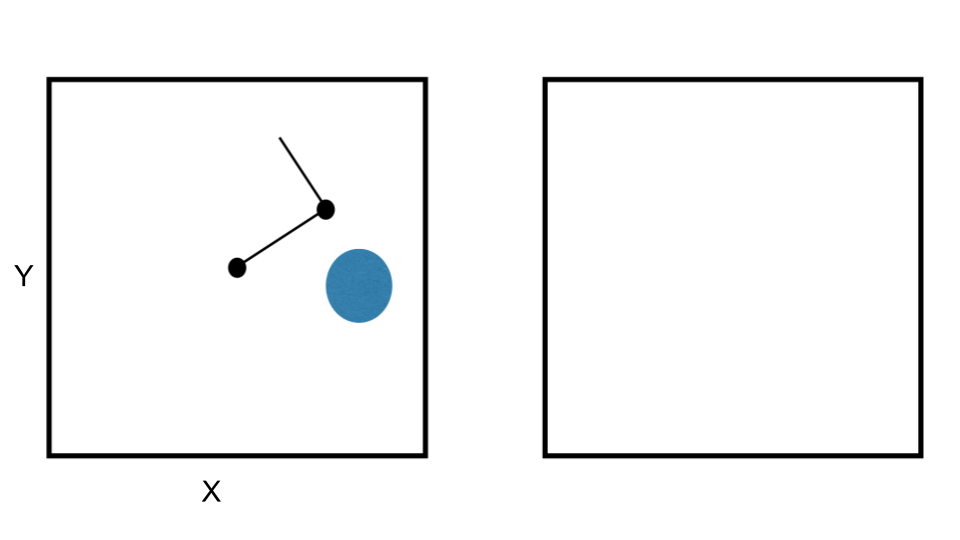
\includegraphics[scale = 0.35, center]{PS3/fig/configSpace.png}

%%%%%%%%%%%%%%%%%%%%%%%%%%%%%%%%%%%%%%%%%%%%%%%%%%%%%%%%%%%%%%%%%%%%%%%%%%%%%%%%%%%%%%%%%%%%%%%%
\clearpage
\textbf{Problem 2: (Optimal) Control (5 points)}\\
Suppose we are trying to control a Cart-Pole to hold the pole upright. Note that the the cart can move left or right along the track and is powered, while the pendulum has no motor ($u \in \mathcal{R}$ and $x\in \mathcal{R}^4 = [x,\theta,\dot{x},\dot{\theta}$]). Assume that we start at $x_0 = [0,\frac{3\pi}{4},0,0]$ and have a goal as mentioned earlier of $x_g = [0,\pi,0,0]$. Finally, assume that the default control input is $0$.

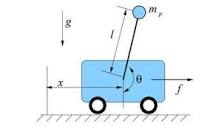
\includegraphics[scale = 0.8, center]{PS3/fig/cartpole.jpeg}

\begin{enumerate}[label=(\alph*)]
    \item What would the feedback control, $u$, be at $x_0$ if we are are using P-Control at the goal with $K_P = [1,4]$.
    \item What would the feedback control, $u$, be at $x_0$ if we are are using PD-Control at the goal with $K_P = [1,4]$ and $K_D = [0.1,0.1]$.
    \item Assume that sometime later we have now moved to the state $[0.1,\frac{7\pi}{8},-1,1]$. Now what would the feedback control be in we are using PD-Control at the goal with $K_P = [1,\frac{8}{\pi}]$ and $K_D = [0.1,0.1]$.
    \item Assume the controller from part (c) overshot the stable upright point. How might you adjust the controller to mitigate that error?
    \item Assume the controller from part (d) had a steady state error. How might you adjust the controller to mitigate that error?
\end{enumerate}

\textbf{Solution 2:}
\begin{enumerate}[label=(\alph*)]
    \item % TODO: Your solution to Problem 2a
    \item % TODO: Your solution to Problem 2b
    \item % TODO: Your solution to Problem 2c
    \item % TODO: Your solution to Problem 2d
    \item % TODO: Your solution to Problem 2e
\end{enumerate}

%%%%%%%%%%%%%%%%%%%%%%%%%%%%%%%%%%%%%%%%%%%%%%%%%%%%%%%%%%%%%%%%%%%%%%%%%%%%%%%%%%%%%%%%%%%%%%%%
\clearpage
\textbf{Problem 3: Machine Learning - Linear Models (5 points)}\\
You are a turnip farmer, and after a few years of tumultuous harvests, you decide to take a quantitative approach to agriculture. You decide to model your annual turnip yield (y) as a linear function of a single variable: the amount of rainfall in the previous year (x) with the following data points:
\begin{table}[ht]
    \center
    \begin{tabular}{|c|c|}
    \hline
    turnip yield (y) & rainfall (x) \\
    \hline
    24 & 10 \\
    \hline
    33 & 14 \\
    \hline
    34 & 12 \\
    \hline
    \end{tabular}
\end{table} \\
Assume your are looking for a parameter $\theta$, and your model is $f_{\theta}(x) = \theta x$.
\begin{enumerate}[label=(\alph*)]
    \item Suppose you are using a quadratic loss function, $L(X, Y) = \sum \left[f_{\theta}(x_i) - y_i\right]^2$, and you can choose $\theta$ to be equal to either 1, 2, or 3. Which is the best option for your data? Why?
    \item Now suppose you are using an $L_1$ loss function, $L(X, Y) = \sum \left|f_{\theta}(x_i) - y_i\right|$, and you can choose $\theta$ to be equal to either 1, 2, or 3. Which is the best option for your data? Why?
    \item Why might the $L_1$ loss function be hard to use in practice? Hint: how do you optimize it and what might go wrong?
\end{enumerate}

\textbf{Solution 3:}
\begin{enumerate}[label=(\alph*)]
    \item % TODO: Your solution to Problem 3a
    \item % TODO: Your solution to Problem 3b
    \item % TODO: Your solution to Problem 3c
\end{enumerate}

%%%%%%%%%%%%%%%%%%%%%%%%%%%%%%%%%%%%%%%%%%%%%%%%%%%%%%%%%%%%%%%%%%%%%%%%%%%%%%%%%%%%%%%%%%%%%%%%
\clearpage
\textbf{Problem 4: Machine Learning - Nonlinear Models (4 points)}\\
You are working for a hospital, and are given a dataset of patient information with hundreds of continuous features (height, weight, blood pressure, etc) along with whether the patient has diabetes -- that is a vector of features $f_i(x)$ for a patient $x$ and the output of whether or not they have the disease $y$. Your goal is to predict whether incoming patients will have diabetes. You decide that logistic regression would be a good way to solve the problem.

\begin{enumerate}[label=(\alph*)]
    \item Assume that you have learned a vector of weights $w$. What equation would you compute to predict if the patient has diabetes. Hint: your answer will be in terms of some subset of $f_i(x), x, y, w$.
    \item Assume you have 200 features and data from only 12 patients. After you have optimized the model (explain each in 1-3 sentences):
    \begin{enumerate}[label=(\roman*)]
        \item How accurate do you think the optimized model will be for those 12 patients?
        \item How accurate do you think the optimized model will be for other patients not in  the dataset?
    \end{enumerate}
    \item Now we are going to use a very large Neural Network instead of logistic regression. Again assume you have 200 features per patient and data from only 12 patients. After you have optimized the model how will the NN model compare to the logistic regression model?
\end{enumerate}

\textbf{Solution 4:}
\begin{enumerate}[label=(\alph*)]
    \item % TODO: Your solution to Problem 4a
    \item \begin{enumerate}[label=(\roman*)]
        \item % TODO: Your solution to Problem 4bi
        \item % TODO: Your solution to Problem 4bii
    \end{enumerate}
    \item % TODO: Your solution to Problem 4c
\end{enumerate}

%%%%%%%%%%%%%%%%%%%%%%%%%%%%%%%%%%%%%%%%%%%%%%%%%%%%%%%%%%%%%%%%%%%%%%%%%%%%%%%%%%%%%%%%%%%%%%%%
\clearpage
\textbf{Problem 5: Convex Optimization (7 Points)}
Answer the following questions about the function:
$$y(x) = \frac{1}{4}x^4 + \frac{1}{3}x^3 - \frac{17}{2}x^2 + 15x + 210$$
\begin{enumerate}[label=(\alph*)]
    \item Compute the derivative $y^\prime(x)$.
    \item What are the critical points of the function?
    \item Show whether each point is a local minima or a local maxima. Hint: you want to compute $y^{\prime\prime}(x)$.
    \item Compute a quadratic approximation $\hat{y}(x)$ of $y(x)$ at $x = 7$.
    \item Starting from that approximation take two gradient \emph{descent} steps using a learning rate of $\alpha = 0.01$. Where do you end up? Hint: you may need to compute a second approximation!
    \item If you were going to do that gradient descent step again starting at $x = 7$ would you increase or decrease the learning rate? Why? Explain in 1-3 sentences.
\end{enumerate}

\textbf{Solution 5:}
\begin{enumerate}[label=(\alph*)]
    \item % TODO: Your solution to Problem 5a
    \item % TODO: Your solution to Problem 5b
    \item % TODO: Your solution to Problem 5c
    \item % TODO: Your solution to Problem 5d
    \item % TODO: Your solution to Problem 5e
    \item % TODO: Your solution to Problem 5f
\end{enumerate}

\end{document}